\documentclass[a4paper, 12pt]{article}

\usepackage[slovene]{babel}
\usepackage[utf8]{inputenc}
\usepackage[T1]{fontenc}
\usepackage{lmodern}
\usepackage{amsmath}
\usepackage{amsfonts}
\usepackage{amssymb}
\usepackage{bbm}
\usepackage{hyperref}
\usepackage{makeidx}
\usepackage[most]{tcolorbox}
\usepackage{graphicx,subfig}
\usepackage{makecell}
\usepackage{longtable}

\usepackage{graphicx}
\graphicspath{{./slike/}} 


\textwidth 15cm
\textheight 24cm
\oddsidemargin.5cm
\evensidemargin.5cm
\topmargin-5mm
\addtolength{\footskip}{10pt}
\pagestyle{plain}
\overfullrule=15pt

% ================================================================================================

\begin{document}
    
\thispagestyle{empty}
\noindent{\large
Univerza v Ljubljani\\[2mm]
Fakulteta za matematiko in fiziko\\[2mm]
Finančna matematika 1.~stopnja}
\vfill

\begin{center}{\large
Projekt pri predmetu Finančni praktikum\\[5mm]
{\Huge \bf The firefighter problem}\\[5mm]
Karolina Šavli in Klara Travnik\\[1cm]}
\end{center}
\vfill

\noindent{\large Ljubljana, januar 2023}
\pagebreak

% ================================================================================================

\tableofcontents

\pagebreak

% ================================================================================================

\section{Opis in formulacija problema}

\subsection{Predstavitev problema}
\noindent \emph{The firefighter problem} oziroma \emph{problem gasilca} je optimizacijski problem, katerega cilj je 
minimiziranje števila pogorelih vozlišč na grafu. \\
Vhodni podatki problema so:
\begin{itemize}
    \item graf $G,$
    \item množica vozlišč $B_{init} \subseteq V\left(G\right)$, na katerih v času $0$ izbruhne požar in
    \item število gasilcev $D$.
\end{itemize} 
V vsaki časovni enoti ($t > 0$) gasilci izberejo nepogorela vozlišča, ki jih bodo rešili tako,
da čim bolj omejijo požar. Ta se lahko razširi le na sosede že pogorelih vozlišč, ki niso še zaščitena. 
V nalednji časovni enoti gasilci ponovno gasijo požar in opisan
proces se ponavlja dokler požar ni zajezen. \\

\noindent Predpostavke problema: 
\begin{itemize}
    \item če je bilo vozlišče v nekem času $t$ rešeno ali je pogorelo, obvelja rešeno oz. pogorelo tudi v 
    vseh prihodnjih časih,
    \item vozlišče $v$ ne more biti hkrati označeno kot pogorelo in rešeno,
    \item v vsakem času $t$ je na voljo fiksno število gasilcev; vsak lahko reši
    eno vozlišče, torej je v vsakem času največ $D$ na novo rešenih.
\end{itemize}

\subsection{Program}
\overfullrule=0pt
\noindent Opisani problem sva v programu \emph{CoCalc}, v programskem jeziku \emph{SageMath} 
zapisali kot \textbf{celoštevilski linearni program (CLP)}: \\

\begin{scriptsize}
\begin{verbatim}
    def clp(G, B, gasilci):
        ''' vhodni podatki:
            G           izbran graf
            B           vozlišča, ki na začetku zgorijo
            gasilci     število gasilcev, ki v vsakem koraku gasijo požar
            izhodni podatki:
            seznam oblike [št. časovnih enot, pogorela/burnt vozlišča po časih, 
                    zaščitena/defended vozlišča po časih] '''
        cas = 10
        while True:
            casi = range(1, cas+1) # uprabljamo pri zankah
        
            # CLP:
            p = MixedIntegerLinearProgram(maximization=False) # CLP
            d = p.new_variable(binary=True) # spremenljivka, defended
            b = p.new_variable(binary=True) # spremenljivka, burnt

            # minimiziramo število pogorelih vozlišč na koncu:
            p.set_objective(sum(b[i, cas] for i in G)) 




            for t in casi:
                for i in G:
                    for j in G[i]: # j je številka v seznamu vozlišča i, sosed od i
                        p.add_constraint(b[i,t] + d[i,t] - b[j,t-1] >= 0)
                    p.add_constraint(b[i,t] + d[i,t] <= 1)
                    p.add_constraint(b[i,t] - b[i,t-1] >= 0)
                    p.add_constraint(d[i,t] - d[i,t-1] >= 0)
                p.add_constraint(sum((d[i,t] - d[i,t-1]) for i in G) <= gasilci)

            for i in G:
                p.add_constraint(b[i,0] == (1 if i in B else 0))
                p.add_constraint(d[i,0] == 0)
                
            k = p.solve()
            l = p.get_values(b)
            m = p.get_values(d)
            
            # Ali je problem končan?
            n = skrcitev(l, cas) # burnt vozlišča v cas
            e = skrcitev(m, cas) # defended vozlišča v cas
            skupaj = n + e
            
            koncan = 1
            # sosedi od pogorelih vozlišč so lahko pogoreli ali zaščiteni. 
            #           Ne smejo biti prazna vozlišča.
            for pogorelo_vozlisce in n:
                for sosed_od_pogorelo_vozlisce in G[pogorelo_vozlisce]:
                    if sosed_od_pogorelo_vozlisce not in skupaj:
                        koncan = 0
            koncan
            
            if koncan == 1:
                break
            else:
                cas += 10
            
        return [k, l, m]\end{verbatim}
\end{scriptsize}

\noindent CLP sva želeli zastaviti tako, da v argumentu funkcije ni potrebno nastaviti časa v
katerem naj bi bil CLP končan. Slednje sva dosegli z \emph{while True} zanko in
nastavitvijo začetnega časa, $cas = 10$. V tem času je problem lahko
končan ali ne. Če problem v tem času ni končan, torej rešitev ni končna, sva čas povečali za $10$ ter
algoritem ponovili.
Da je rešitev končna pomeni, da za vsako vozlišče, ki je zgorelo, velja, da je vsako sosednje
vozlišče le-tega tudi zgorelo, ali pa že rešeno/pogašeno. \\

\noindent Za število potrebnih časovnih korakov, da dobimo končno rešitev (torej da se proces/situacija 
v naslednjih časih ne spreminja),
sva napisali naslednjo funkcijo:

\begin{scriptsize}
\begin{verbatim}
    def cas_potreben(G, B, gasilci):
        ''' iz p.solve() pridobi čas po katerem se nič več ne spremeni -> dobimo potreben čas '''
        cas = 10
        while True:
            t, burnt, defended = clp(G, B, gasilci)

            # uredi glede na čas naraščajoče:
            urej_burnt = sorted(burnt.items(), key=lambda tup: tup[0][1])
            urej_defended = sorted(defended.items(), key=lambda tup: tup[0][1]) 

            vredn_burnt= []
            for i, v in urej_burnt:
                vredn_burnt.append(v)
            # pridobim ven vrednosti spremnljivk b v časih in vozliščih naraščajoče

            vredn_defended= []
            for i, v in urej_defended:
                vredn_defended.append(v)
            # pridobim ven vrednosti spremnljivk d v časih in vozliščih naraščajoče

            # from itertools import islice
            from itertools import accumulate
            dolzina = [len(G)] * (cas +1) # Vrednosti zgrupiram v paketke, 
                                          # v vsakem je toliko vrednosti, kolikor je vozlišč
            seznami_vrednosti_po_casih_burnt = [tuple(vredn_burnt[x - y: x]) for x, y in zip(
                                accumulate(dolzina), dolzina)]

            seznami_vrednosti_po_casih_defended = [tuple(vredn_defended[x - y: x]) for x, y in zip(
                                accumulate(dolzina), dolzina)]

            d = next(i for i in range(len(dolzina)) 
                if all(len(set(l[i:i+2])) == 1 
                for l in (seznami_vrednosti_po_casih_burnt, seznami_vrednosti_po_casih_defended)))
            if d < cas:
                break
            else:
                cas += 10
        return d\end{verbatim}
\end{scriptsize}

\noindent Funkcija $cas\_potreben$ torej za vsak graf, podmnožico vozlišč $B$ grafa ter določeno število gasilcev
izračuna potreben čas za rešitev algoritma. \\
Opomba: potreben čas ni enak časovni zahtevnosti
algoritma. Potreben čas predstavlja število časovnih enot v procesu širjenja požara in reševanju vozlišč.
Časovno zahtevnost pa bova obravnavali v nadaljevanju. 

\pagebreak

% ================================================================================================
% ================================================================================================

\section{Vizualizacija problema}

\subsection{Predstavitev funkcij za barvanje}

\noindent Za lažjo predstavo poteka problema sva napisali funkcijo $barvanje\_po\_korakih$, ki z barvanjem
vozlišč grafa prikazuje širjenje in zajezevanje požara. Koda funkcije je naslednja:

\begin{scriptsize}
\begin{verbatim}
    def barvanje_v_casu_t(G, B, gasilci, t):
        ''' pomožna funkcija barvanje_v_casu_t izriše graf in pobarva vozlišča v določenem času (t). 
            Začetna vozlišča oz. izvor pošara pobarva v zeleno, 
            pogorela v  rdečo, zaščitena pa v modro. '''
        b = skrcitev(clp(G, B, gasilci)[1], t) # burnt vozlišča v času t BREZ ZAČETNIH VOZLIŠČ B
        for el in B:
            b.remove(el)
        d = skrcitev(clp(G, B, gasilci)[2], t) # defended vozlišča v času t
        
        return G.show(partition = [b, B, d])


    def barvanje_po_korakih(G, B, gasilci):
        ''' funkcija, ki za vsako časovno enoto nariše situacijo na grafu
            barve:
                - zelena: oglišča kjer se požar začne (B)
                - rdeča: pogorela
                - modra: zaščitena '''
        time = cas_potreben(G, B, gasilci)
        print("Število potrebnih časovnih korakov: " + str(time))
        for t in range(0, time + 1):
            print("Situacija v času " + str(t) + ":")
            barvanje_v_casu_t(G, B, gasilci, t)\end{verbatim}
\end{scriptsize}

\noindent Funkcija $barvanje\_po\_korakih$ deluje s pomočjo funkcije $barvanje\_v\_casu\_t$, ki predstavlja
situacijo na grafu v času t, torej katera vozlišča so pogorela in katera zaščitena.
 Funkcijo si za lažje razumevanje poglejmo na konkretnem primeru.

\subsection{Primer na Petersonovem grafu}
\noindent Potek problema in barvanje predstavimo na Petersonovem grafu. \\ 
Funkcija $barvanje\_po\_korakih$ zahteva tri argumente
in sicer graf $G$, množico izvornih vozlišč $B$ ter $gasilci$, ki predstavlja število gasilcev, ki 
bodo v vsaki časovni enoti gasili požar.
Izberemo si naslednje:
\begin{small}
\begin{verbatim}
    G = graphs.PetersenGraph()
    B = [1, 5]
    gasilci = 2
\end{verbatim}
\end{small}
Imamo torej Petersonov graf, na katerem bo požar izbruhnil v vozliščih $1$ in $5$ in v vsaki časovni enoti ga bosta
gasila dva gasilca. \\
Opomba: množico vozlišč $B$ bi lahko izbrali tudi naključno in sicer s funkcijo, ki bo predstavljana
v nadaljevanju, in za aragument prejme graf ter število vozlišč, ki bi radi da so izvor požara. 
Vrne pa naključna vozlišča grafa. \\

\noindent Če zaženemo
\begin{small}
\begin{verbatim}
    barvanje_po_korakih(G2, B2, gasilci2)
\end{verbatim}
\end{small}
dobimo naslednje:
\begin{small}
\begin{verbatim}
    Število potrebnih časovnih korakov: 2
    Situacija v času 0:
\end{verbatim}
\end{small}
    \begin{center}
        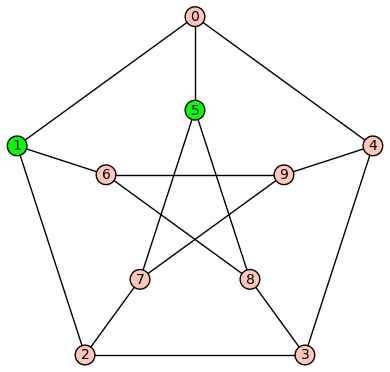
\includegraphics[scale=0.5]{peterson0}
    \end{center}
\begin{small}
\begin{verbatim}
    Situacija v času 1:
\end{verbatim}
\end{small}
    \begin{center}
        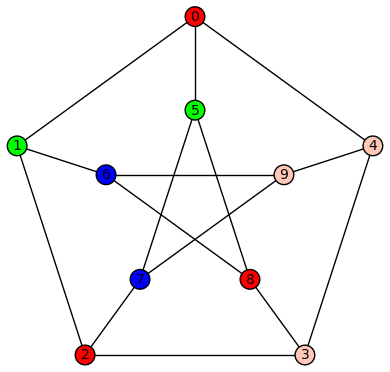
\includegraphics[scale=0.5]{peterson1}
    \end{center}
\begin{small}
\begin{verbatim}
    Situacija v času 2:
\end{verbatim}
\end{small}
    \begin{center}
        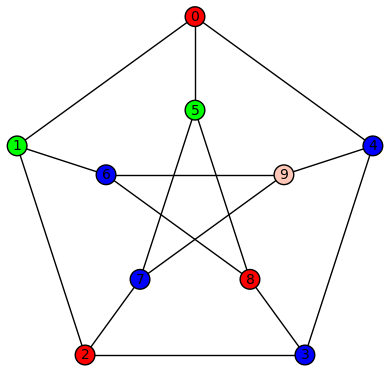
\includegraphics[scale=0.5]{peterson2}
    \end{center}

\noindent Funkcija $barvanje\_po\_korakih$ nam na začetku izpiše število potrebnih 
časovnih korakov, ki jih izračuna z že predstavljeno funkcijo $cas\_potreben$. 
Nato pa nam izriše situacijo v vsakem časovnem koraku:
\begin{itemize}
    \item situacija \underline{v času $0$} so
    zgolj vozlišča izvora požara, v našem primeru vozlišči $1$ in $5$. \textcolor{green}{Vozlišča izvora} 
    požara so tekom celotne grafične predstavitve pobarvane v \textcolor{green}{zeleno}. 
    \item v naslednjem časovnem koraku, \underline{času $1$} dva gasilca zaščitita požar in sicer v vozlišču $6$ in $7$.
    \textcolor{blue}{Zaščitena vozlišča} so pobarvana z \textcolor{blue}{modro}. Po tem ko gasilca zaščitita omenjeni vozlišči, se
    požar lahko naprej razširi le v vozlišče $2$ in $0$ (iz že zagorelega vozlišča $1$) ter v vozlišče $8$ (iz že
    zagorelega vozlišča $5$). \textcolor{red}{Pogorela vozlišča} so pobarvana z \textcolor{red}{rdečo}.
    \item v naslednjem času, \underline{času $2$} gasilca ponovno zaščitita vozlišči in sicer $3$ ter $4$. 
    Z grafičnega prikaza je razvidno, da se požar ne more več razširiti naprej. Edino nepogorlo
    in nezaščiteno vozlišče pa je vozlišče $9$.
\end{itemize}

\pagebreak

% ================================================================================================

\section{Časovna zahtevnost}
\overfullrule=0pt

Kot zanimivost sva s pomočjo \emph{Python} knjižnice \emph{timeit} generirali funkcijo, ki nam 
vrne časovno zahtevnost funkcije $clp$, opisane v prvem poglavju. 
Kot že znano, funkcija $clp$ sprejme tri argumente: graf, množico izvorov požara in
število gasilcev. Funkciji sva podali poljuben graf, naključno vozlišče (eno samo) ter
določili sva, da bo požar gasil samo en gasilec.
Slednje sva naredili na grafih s številom vozlišč iz množice $ \left\{ 6, 8, 10, 12, \ldots 98, 100 \right\} $.
Dobljene rezultate sva predstavili v grafu: \\

\begin{center}
    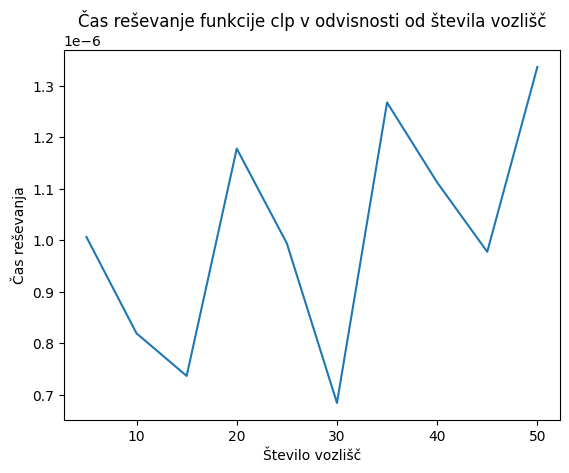
\includegraphics[scale=0.7]{cas}
\end{center}

\noindent Opazimo, da časovna zahtevnost reševanja funckije $clp$ za najine primere ni v očitni relaciji s
številom vozlišč.
Opaziti pa je, da se časovna zahtevnost vendarle počasi povečuje z večanjem števila vozlišč 
grafa.
Predvidevava, da je časovna zahtevnost v splošnem večja za grafe z večjim 
številom vozlišč ter večjo množico začetnih gorišč, saj je tudi število časovnih korakov do zaključenega problema v
tem primeru večje. Predvidevanje bi lahko potrdile (ali ovrgle) s simulacijo, ki bi jo izvedle
na podoben način kot testiranje v naslednjem poglavju.

\pagebreak

% ================================================================================================
\overfullrule=0pt
\section{Testiranje programa glede na število vozlišč grafa}

\subsection{Potek dela}

Za izvedbo testiranja programa sva spisali funkcijo $seznam\_naborov\_st\_vozlisc\_cas$, ki
kot argumente sprejme $seznam\_imen\_grafov$, $st\_gasilcev$ ter $stevilo\_vozlic\_v\_B$. Tekom
funkcije se sprehodimo čez $seznam\_imen\_grafov$ (seznam poljubnih imen grafov) in sestavljamo 
nov seznam sestavljen iz naborov oblike  
$$\left( \text{število vozlišč grafa}, \text{potreben čas reševanje problema na grafu} \right).$$
Koda funkcije:

\begin{scriptsize}
\begin{verbatim}
    import random
    def nakljucno_izberi_vzolisca(graf, n):
        ''' funkcija naključno izbere n vozlišč iz grafa graf '''
        return random.sample(list(graf), n)

    def seznam_naborov_st_vozlisc_cas(seznam_imen_grafov, st_gasilcev, stevilo_vozlisc_v_B):
        ''' funkcija, ki sprejme seznam v katerem so imena grafov, število gasilcev ter število vozlišč, 
            ki jih želimo v začetni množici B.
            Vrne pa seznam naborov oblike (število vozlišč, potreben čas reševanje problema)'''
        # sprehodimo se po seznam_imen_grafov in sestavljamo nabor:
        seznam_naborov = []
        for graf in seznam_imen_grafov:
            B1 = nakljucno_izberi_vzolisca(graf, stevilo_vozlisc_v_B)
            B2 = nakljucno_izberi_vzolisca(graf, stevilo_vozlisc_v_B)
            potreben_cas1 = cas_potreben(graf, B1, st_gasilcev)
            potreben_cas2 = cas_potreben(graf, B2, st_gasilcev)
            seznam_naborov.append((len(graf), potreben_cas1))
            seznam_naborov.append((len(graf), potreben_cas2))
        
        return seznam_naborov\end{verbatim}
\end{scriptsize}

\noindent V funkciji sva si pomagali s funkcijo $nakljucno\_izberi\_vozlisca$, ki kot 
argument sprejme poljuben graf $graf$ ter poljubno pozitivno število $n$. Funkcija vrne 
$n$ poljubnih vozlišč $graf$-a. Namen funkcije pa je generiranje naključne množice začetnih 
vozlišč $B$, saj požar lahko izbruhne kjerkoli. \\

\noindent Funkcijo $seznam\_naborov\_st\_vozlisc\_cas$ sva izvedli na zelo velikem seznamu grafov. Grafi seznama
so bili različnih velikosti in oblik. Obravnavo rezultatov sva razdelili glede 
na spremenljivki $st\_gasilcev$ ter $stevilo\_vozlic\_v\_B$. \\
Ločili sva primera:
\begin{itemize}
    \item $st\_gasilcev = 1$ in $stevilo\_vozlic\_v\_B = \left\{ 2, \, 3, \, 4 \right\}$
    \item $st\_gasilcev = 2$ in $stevilo\_vozlic\_v\_B = \left\{ 2, \, 3, \, 4 \right\}$
\end{itemize}

\noindent Iz dobljenih podatkov sva nato sestavili \emph{.csv} datoteko in podatke vizualzirali s pomočjo \emph{Python} knjižnice \emph{pandas}. 
V grobem sva predstavlili odvisnost časa reševanja problema od števila vozlišč grafa. Število vozlišč obravnanih grafov
je med $6$ in $77$. Grafične prikaze sva nazadnje nadgradili še z linarno regresijo. 

\pagebreak

\subsection{1 gasilec \& 2, 3 ali 4 izvori požara}

Za parametre $st\_gasilcev = 1$ in $stevilo\_vozlic\_v\_B = \left\{ 2, \, 3, \, 4 \right\}$ sva dobili
naslednje grafične prikaze:

\begin{figure}[!htb]
    \minipage{0.32\textwidth}
      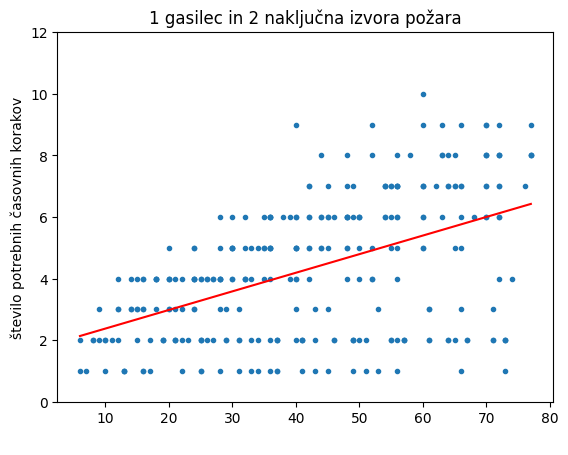
\includegraphics[width=\linewidth]{plot12}
    \endminipage\hfill
    \minipage{0.32\textwidth}
      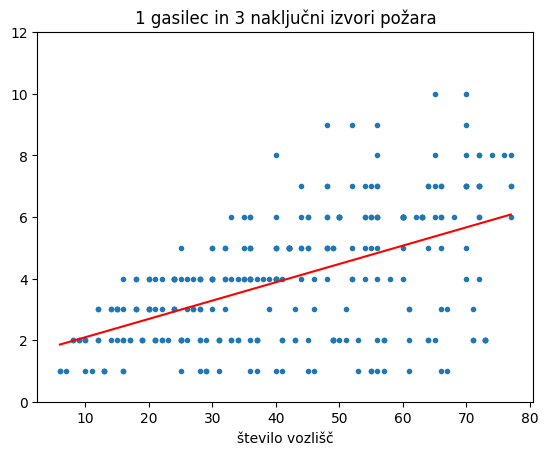
\includegraphics[width=\linewidth]{plot13}
    \endminipage\hfill
    \minipage{0.32\textwidth}
      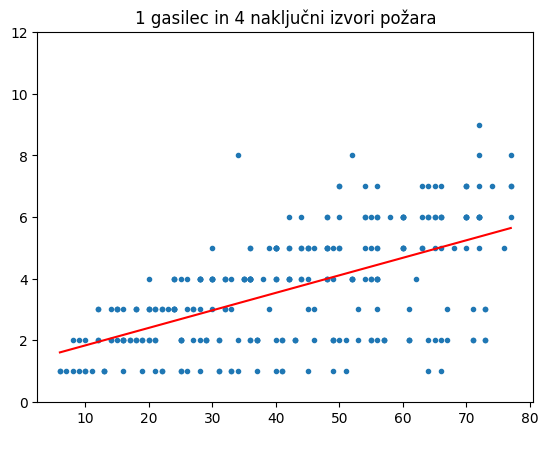
\includegraphics[width=\linewidth]{plot14}
    \endminipage
\end{figure}
    
\noindent Dodatno sva izračunali še povprečno število potrebnih časovnih korakov:
\begin{itemize}
    \item 1 gasilec in 2 naključna izvora požara: $4.304$,
    \item 1 gasilec in 3 naključni izvora požara: $3.993$,
    \item 1 gasilec in 4 naključni izvora požara: $3.645$.
\end{itemize}

\noindent Tako iz grafov kot tudi iz izračuna je razvidno, da se število potrebnih časovnih korakov
z višanjem števila izvorov požara veča. To seveda ni presenetljivo, saj bo $1$ gasilec zagotovo
potreboval več časa za omejitev $4$ izvorov požara, kot na primer $2$ izvorov požara. \\

\noindent Komentar: opazimo, da so dobljena povprečja precej majhna. Slednje si lahko razlagamo z dejstvom, da je bilo v
seznamu grafov več grafov z manjšim številom vozlišč (manj kot $40$). Slednji grafi pa
za zaključek problema potrebujejo manj časa kot grafi z večjim število vozlišč. 

\subsection{2 gasilca \& 2, 3 ali 4 izvori požara}

Za parametre $st\_gasilcev = 2$ in $stevilo\_vozlic\_v\_B = \left\{ 2, \, 3, \, 4 \right\}$ sva dobili
naslednje grafične prikaze:

\begin{figure}[!htb]
    \minipage{0.32\textwidth}
      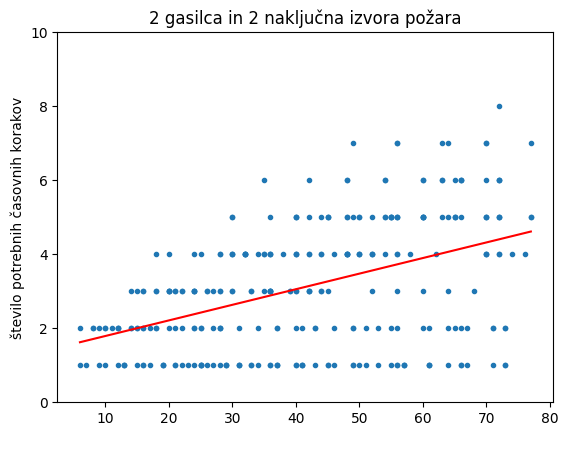
\includegraphics[width=\linewidth]{plot22}
    \endminipage\hfill
    \minipage{0.32\textwidth}
      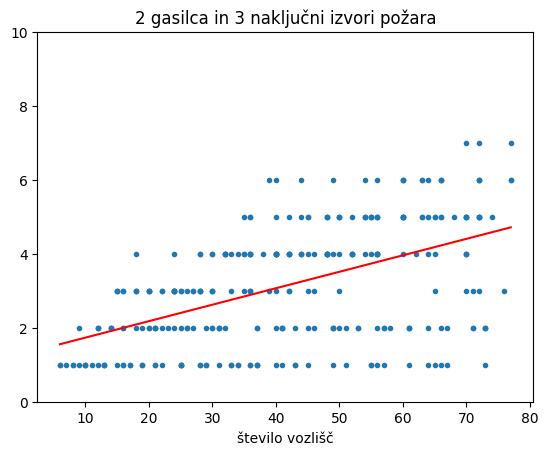
\includegraphics[width=\linewidth]{plot23}
    \endminipage\hfill
    \minipage{0.32\textwidth}
      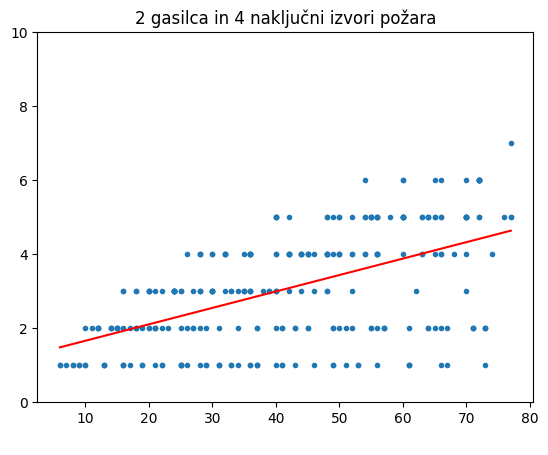
\includegraphics[width=\linewidth]{plot24}
    \endminipage
\end{figure}

\pagebreak

\noindent Dodatno sva izračunali še povprečno število potrebnih časovnih korakov:
\begin{itemize}
    \item 2 gasilca in 2 naključna izvora požara: $3.121$,
    \item 2 gasilca in 3 naključni izvora požara: $3.151$,
    \item 2 gasilca in 4 naključni izvora požara: $3.164$.
\end{itemize}

\noindent V tem primeru pridemo do podobnega sklepa kot v prejšnjem (1 gasilec omejuje požar):
število potrebnih časovnih korakov se z višanjem števila izvorov požara veča. 

\subsection{Primerjava primerov z 1 gasilcem in 2 gasilci}
Primerjamo grafe in razultate, ki smo jih dobili v prejšnjih dveh primerih.
Z grafa in tudi iz povprečji je opazno, da je število potrebnih časovnih enot manjše v primeru, ko
imamo $2$ gasilca, saj večje število gasilcev prej omeji požar. 

% ================================================================================================
\pagebreak
\section{Zaključek}

V praksi najdemo več različic obravnavanega optimizacijskega problema gasilca. Na primer:
\begin{itemize}
    \item\textbf{širjenje bolezni} v manjši skupnosti, kjer z vozlišči grafa predstavimo ljudi 
    in s povezavami stike z drugimi. Če je vozlišče v grafu okuženo, ostane nalezljivo 
    za $A$ časovnih enot in lahko okuži sosede v tem časovnem okviru. Gasilce pa v tem
    primeru nadomestijo ukrepi proti širjenju (e.g. razkuževanje, nošenje mask, ...).
    \item V igri \textbf{policistov in roparja} rešujemo problem, ali lahko $D$ policistov ujame roparja, ki se 
    premika po povezavah grafa. 
    \item Podobnost pa lahko najdemo tudi pri vzpostavljanju \textbf{komunikacijske mreže med člani uporniškega gibanja}
    tako, da se minimizira število izdaj članov.
\end{itemize}

\noindent Delo najinega projekta zajema reševanje, obravnavo in uporabo celoštevilskega linearnega programa. 
Pri slednjem sva si pomagali s članki ``García-Martínez, Blum, Rodríguez in Lozano''\cite{garcia2015} ter
``Fomin, Heggernes in van Leeuwen''\cite{fomin2015}. \\
Problema bi se pa seveda lahko lotili še
na kakšen drug način. V vsakem časovnem koraku iteracije bi lahko na primer kot rešeno označili vozlišče z 
največjo stopnjo. Tako bi preprečili (v primeru da zagori), da se ogenj razširi na sosednja vozlišča
le-tega. V nasprotnem primeru bi bila zajezitev požara težja. 
S takim načinom bi potem morali pri testiranju pogledati razmerje med najvišjo stopnjo 
grafa in časom. Vendar pa na tak način najverjetneje ne bi dobili najboljše
rešitve, kot pri linearnem programu. \\

\noindent Glavni sklepi obravnave \emph{The firefighter problem}:
\begin{itemize}
    \item potreben čas reševanje problema se na splošno linearno povečuje
            v odvisnosti od število vozlišč obravnavanega grafa,
    \item čim več gasilcev gasi požar, čim prej bo problem končan in
    \item čim večje je število izvorov požara, tem slabša bo rešitev linearnega problema 
        (manj nepogorelih vozlišč).
\end{itemize}

\pagebreak
 
\bibliographystyle{plain}
\bibliography{literatura}

% ================================================================================================

\end{document}